\section{Stereoskopische Analyse des Krebsnebels}
\label{sec:analyse}

\subsection{Datenselektion und -rekonstruktion}

Abbildung~\ref{fig:analysischain} zeigt den typischen Ablauf einer
stereoskopischen Analyse mit MAGIC Daten. Die hierzu verwendeten Programme sind
eingebettet in das Softwarepaket MARS (MAGIC analysis and reconstruction
software). In einem ersten Schritt durchlaufen die
Rohdaten der beiden Teleskope eine \textbf{Vorprozessierung}. Dazu gehören die
Zeit- und Ladungskalibrierung der einzelnen Pixel der Kamera mit dem Programm
\textit{sorcerer}, sowie das Image Cleaning und die Parametrisierung des
Kamerabildes mit dem Programm \textit{star}. Beim Image Cleaning wird Rauschen
aus dem Kamerabild entfernt, indem nur die Pixel der Kamera berücksichtigt
werden, die eine bestimmte Signalstärke gemessen haben. Dabei ist die geforderte
Signalstärke auch davon abhängig, ob Pixel in direkter Nachbarschaft
berücksichtigt worden sind. Nach der Reinigng des Kamerabildes wird die
detektierte Form durch Größen, wie zum Beispiel den Schwerpunkt, die Länge und
Breite und den Abstand des Schwerpunktes zum anvisierten Ziel parametrisiert.
Im Anschluss daran werden die Daten der Teleskope durch die Software
\textit{superstar} kombiniert und Stereoparameter für die weitere Analyse
berechnet.

\begin{figure}
  \centering
  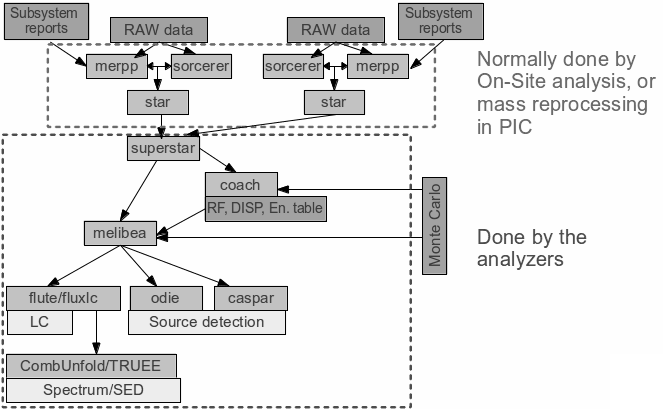
\includegraphics[width=0.9\textwidth]{figures/analysischain.png}
  \caption{Ablauf einer typischen stereoskopischen Analyse mit MAGIC Daten. In
  der hier durchgeführten Analyse wurde mit den Programmen \textit{coach},
  \textit{melibea}, \textit{flute}, \textit{odie}, \textit{caspar} und
  \textit{CombUnfold} gearbeitet \cite{magic_wiki}.} % Referenz: MAGIC wiki
  \label{fig:analysischain}
\end{figure}

In einem nächsten Schritt findet die \textbf{Datenselektion} statt. Der Schritt
ist wichtig, um sicherzustellen, dass die verwendeten Daten vergleichbar und
nicht durch äußere Einflüsse verfälscht sind. Somit dient die Selektion der
Qualitätssicherung der Daten. Für die weitere Analyse werden nur Daten
weiterverwendet, die den folgenden Kriterien genügen:
\begin{itemize}
  \item ...
  \item ...
  \item ...
\end{itemize}
[...Begründung für die Wahl der Kriterien...]

Als nächstes wird das Programm \textit{coach} (Compressed Osteria Alias
Computation of the Hadroness parameter) verwendet, um Modelle für die
\begin{enumerate}
  \item Separation von Gamma- und Hadronenstrahlung,
  \item Energieabschätzung und
  \item Positionsrekonstruktion
\end{enumerate}
aufzustellen. Dies ist notwendig, um das beobachtete Signal klassifizieren zu
können. Die Unterscheidung von Gamma- und Hadronenstrahlung ist möglich, da die
Wahrscheinlichkeit für die Interaktion eines Hadrons mit den Molekülen der
Atmosphäre kleiner ist als die elektromagnetische Interaktion von Gammastrahlung
mit dieser. Daraus resultierend fliegen Hadronen in einem Schauer weiter und der
Schauer ist weiter gefächert als eine elektromagnetischer Schauer.
Abbildung~\ref{fig:gamma_hadron} zeigt den Unterschied der Form eines
hadronischen und eines elektromagnetischen Schauers. Zur Klassifikation wird ein
\textit{random forest} verwendet. Dieser wird trainiert mit einem Teil des
Datensatzes und einem Monte Carlo generierten Datensatz, der auf Grundlage eines
Modells generiert wurde, welches durch Gammastrahlung induzierte Teilchenschauer
beschreibt. Um die Trennkraft des Klassifizierers zu testen wird der Monte
Carlo Datensatz zu Beginn in einen Test- und einen Trainingsdatensatz
aufgeteilt. Somit ist es möglich mit einem Teil des Datensatzes den
Klassifizierer zu trainieren und mit dem anderen Teil zu testen.

\begin{figure}
  \centering
  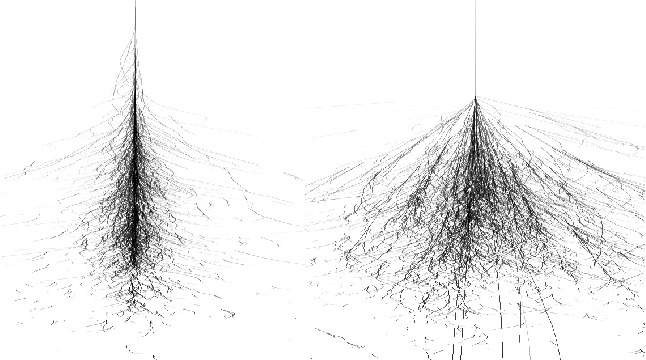
\includegraphics[width=0.7\textwidth]{figures/gamma_hadron.png}
  \caption{Struktur eines elektromagnetischen (links) und eines hadronischen
  (rechts) Schauers. Da Hadronen mit geringer Wahrscheinlichkeit mit der
  Atmospähre wechselwirken als Elektronen und Photonen, fliegen sie weiter und
  der Schauer fächert weiter auf.}
  \label{fig:gamma_hadron}
\end{figure}

Für die Energierekonstruktion werden sogenannte \textit{lookup tables} (LUTs)
generiert, durch die eine Abschätzung der Energie aufgrund der Korrelation
zwischen den Bildparametern und der Stärke des Signals erfolgt.

Nachdem die Modelle erstellt wurden, werden diese mit dem Programm
\textit{melibea} auf den vollständigen Datensatz angewendet. Mit dem nun fertig
präparierten Datensatz können im letzten Analyseschritt Physikresultate
produziert werden.

\subsection{Ergebnisse der Analyse}

Abbildung~\ref{fig:skyplot} (auch \textit{skyplot} genannt) zeigt den mit dem
Programm \textit{casper} berechneten relativen Fluss aufgetragen gegen die
Position am Himmel. Die eingezeichnete \textit{point spread function} (PSF)
veranschaulicht, die Detektorantwort des Teleskops auf eine punktförmige Quelle
am Himmel und ist somit ein Maß für die Auflösung des Teleskops. Es zeigt sich,
dass der Krebsnebel für das Teleskop eine Punktquelle darstellt.

\begin{figure}
  \centering
  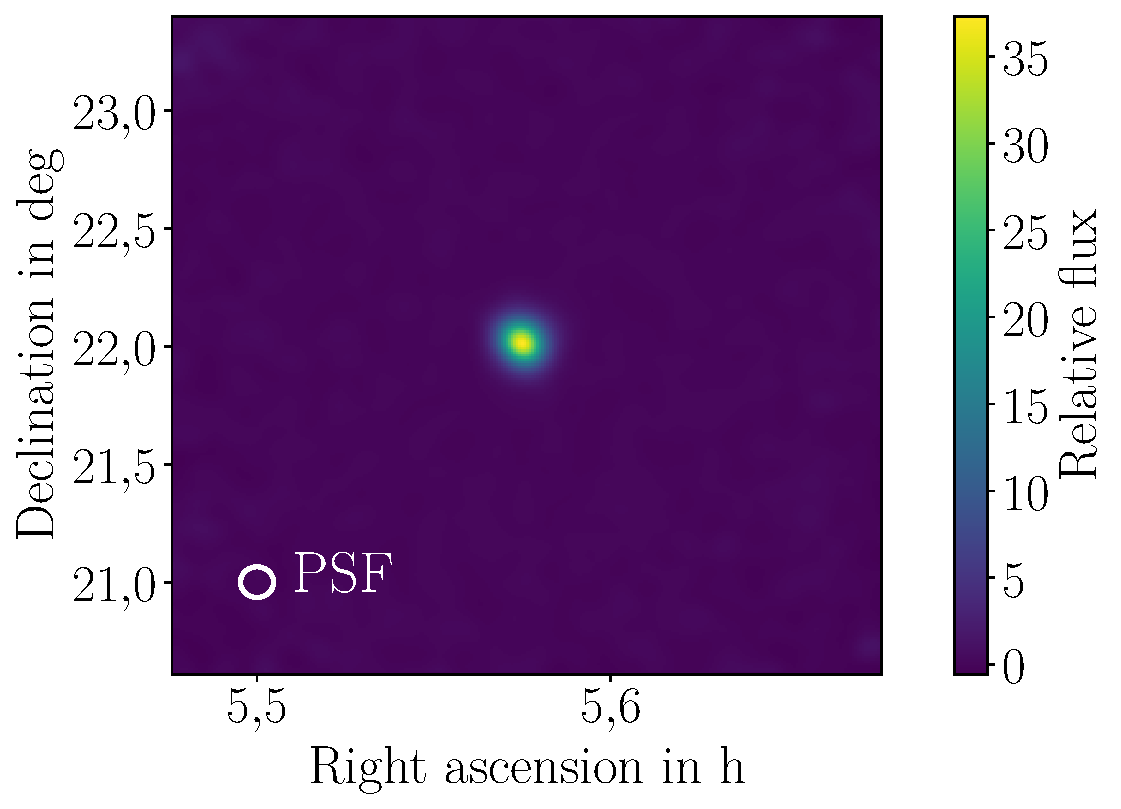
\includegraphics[width=0.8\textwidth]{figures/caspar_flux_skymap.pdf}
  \caption{Veranschaulichung des relativen Flusses in Abhängigkeit von der
  Position am Himmel. Die eingezeichnete Ellipse stellt die
  \textit{point spread function} (PSF) und ist ein Maß für die Auflösung des
  Teleskops.}
  \label{fig:skyplot}
\end{figure}

\begin{figure}
  \centering
  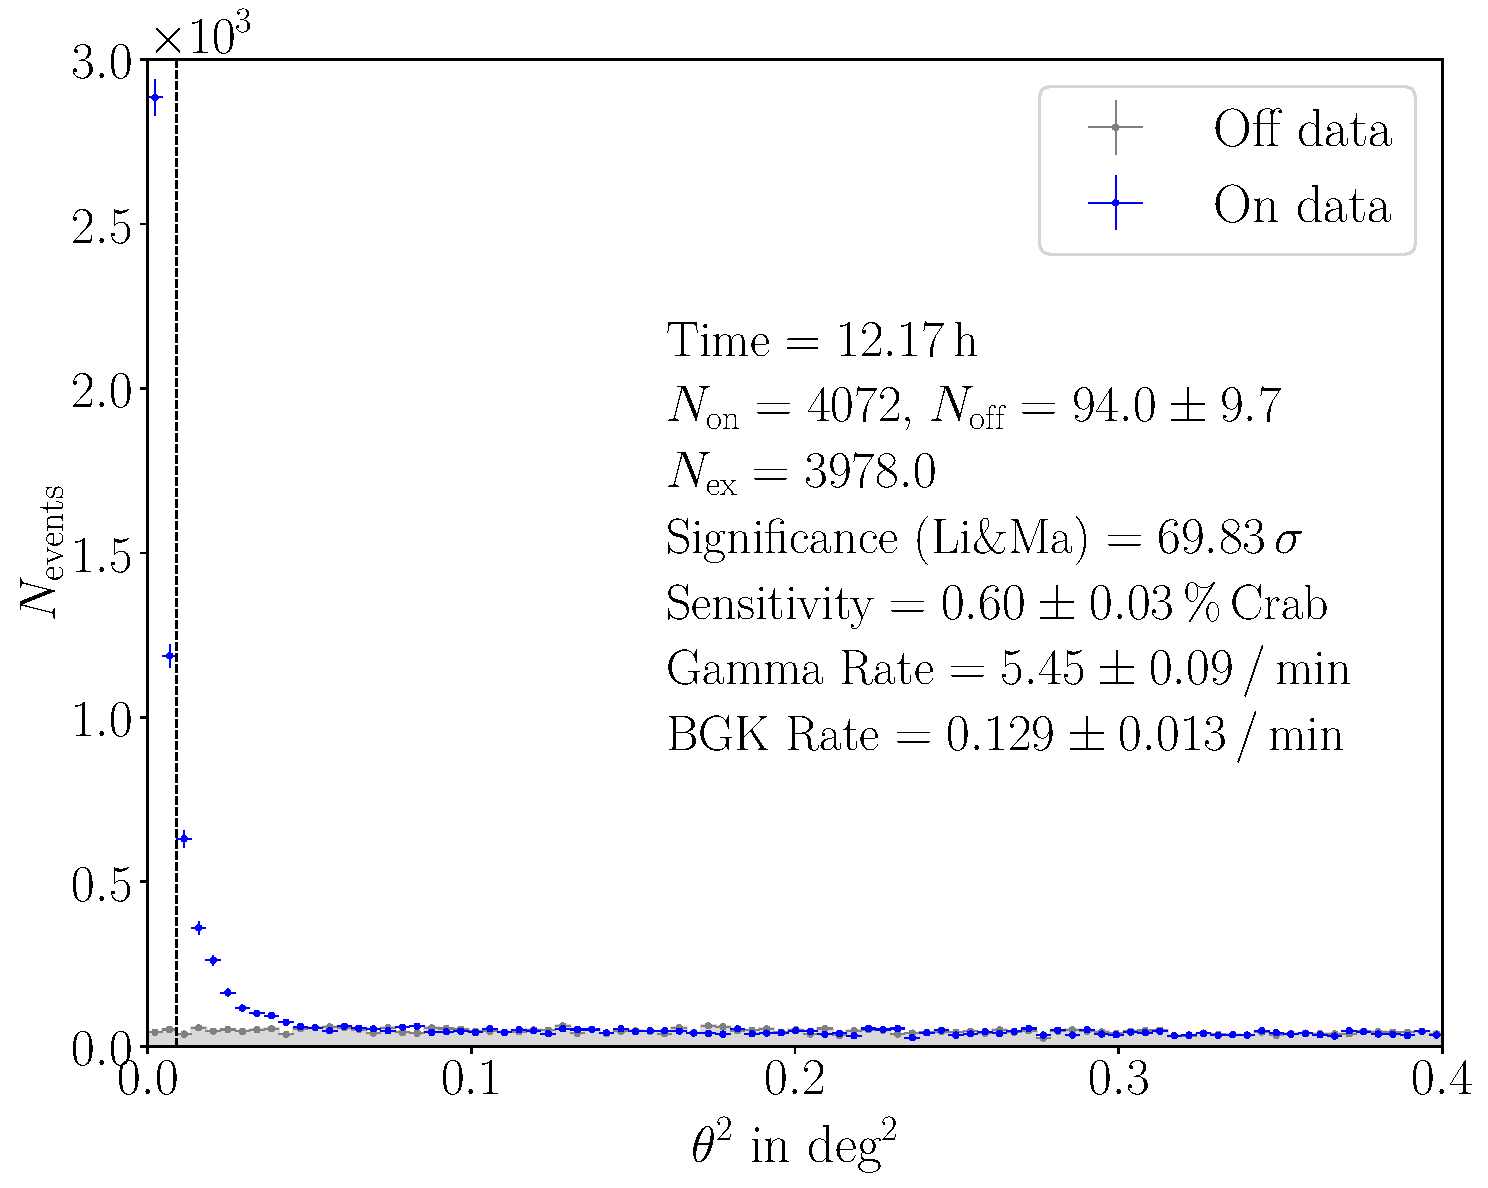
\includegraphics[width=0.8\textwidth]{figures/odie_thetasquared.pdf}
  \caption{Eine Caption.}
\end{figure}

\begin{figure}
  \centering
  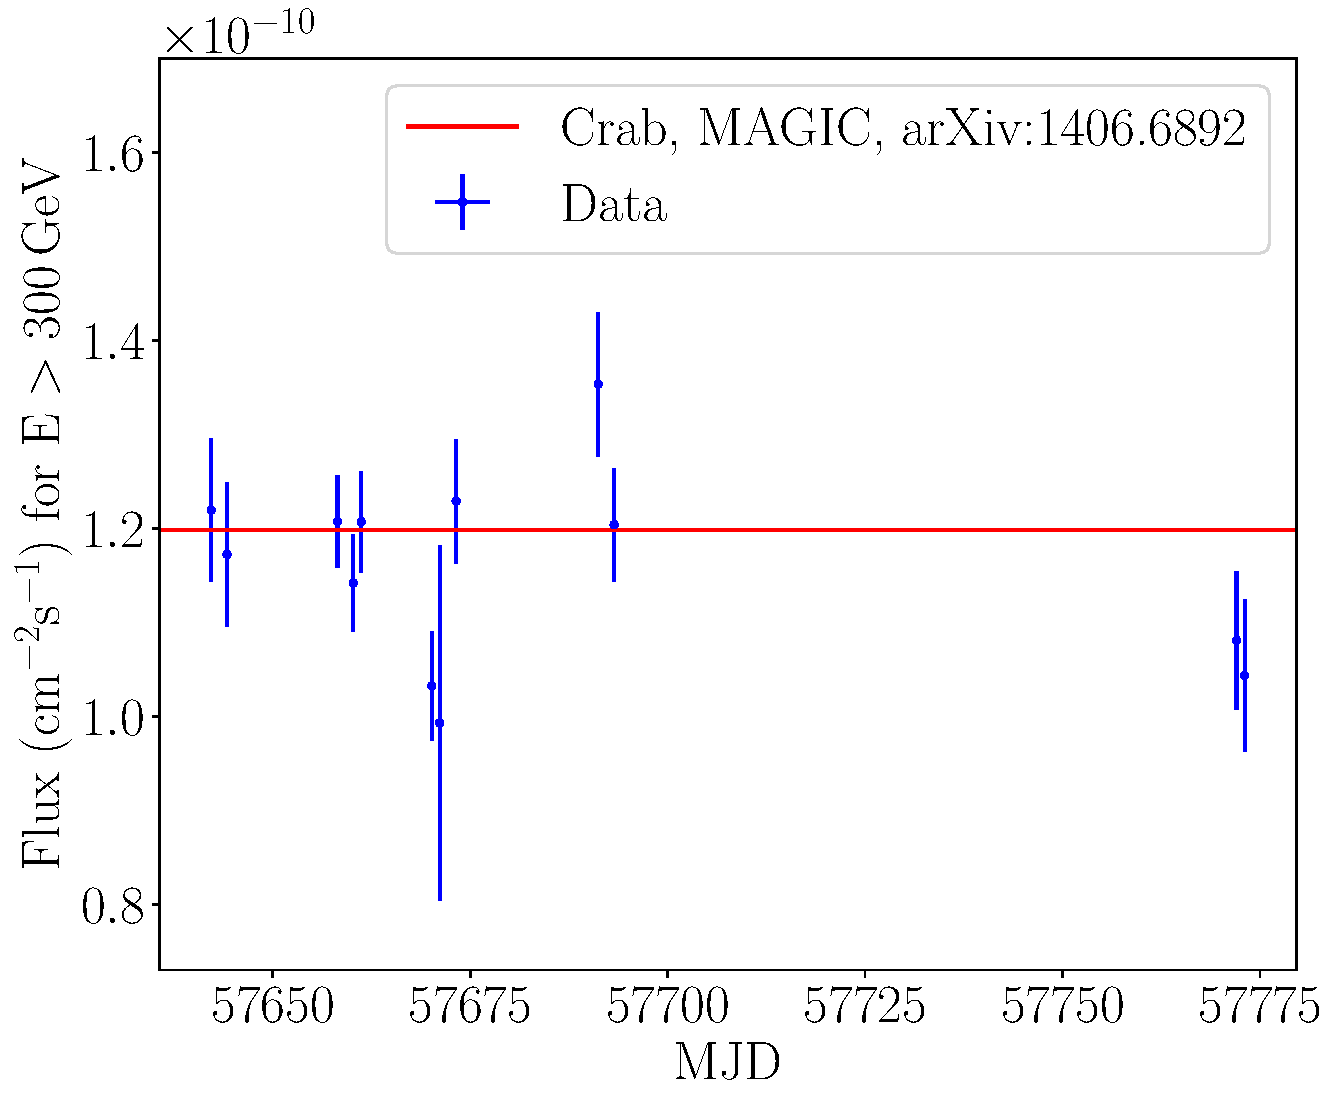
\includegraphics[width=0.8\textwidth]{figures/flute_lichtkurve.pdf}
  \caption{Eine Caption.}
\end{figure}

\begin{figure}
  \centering
  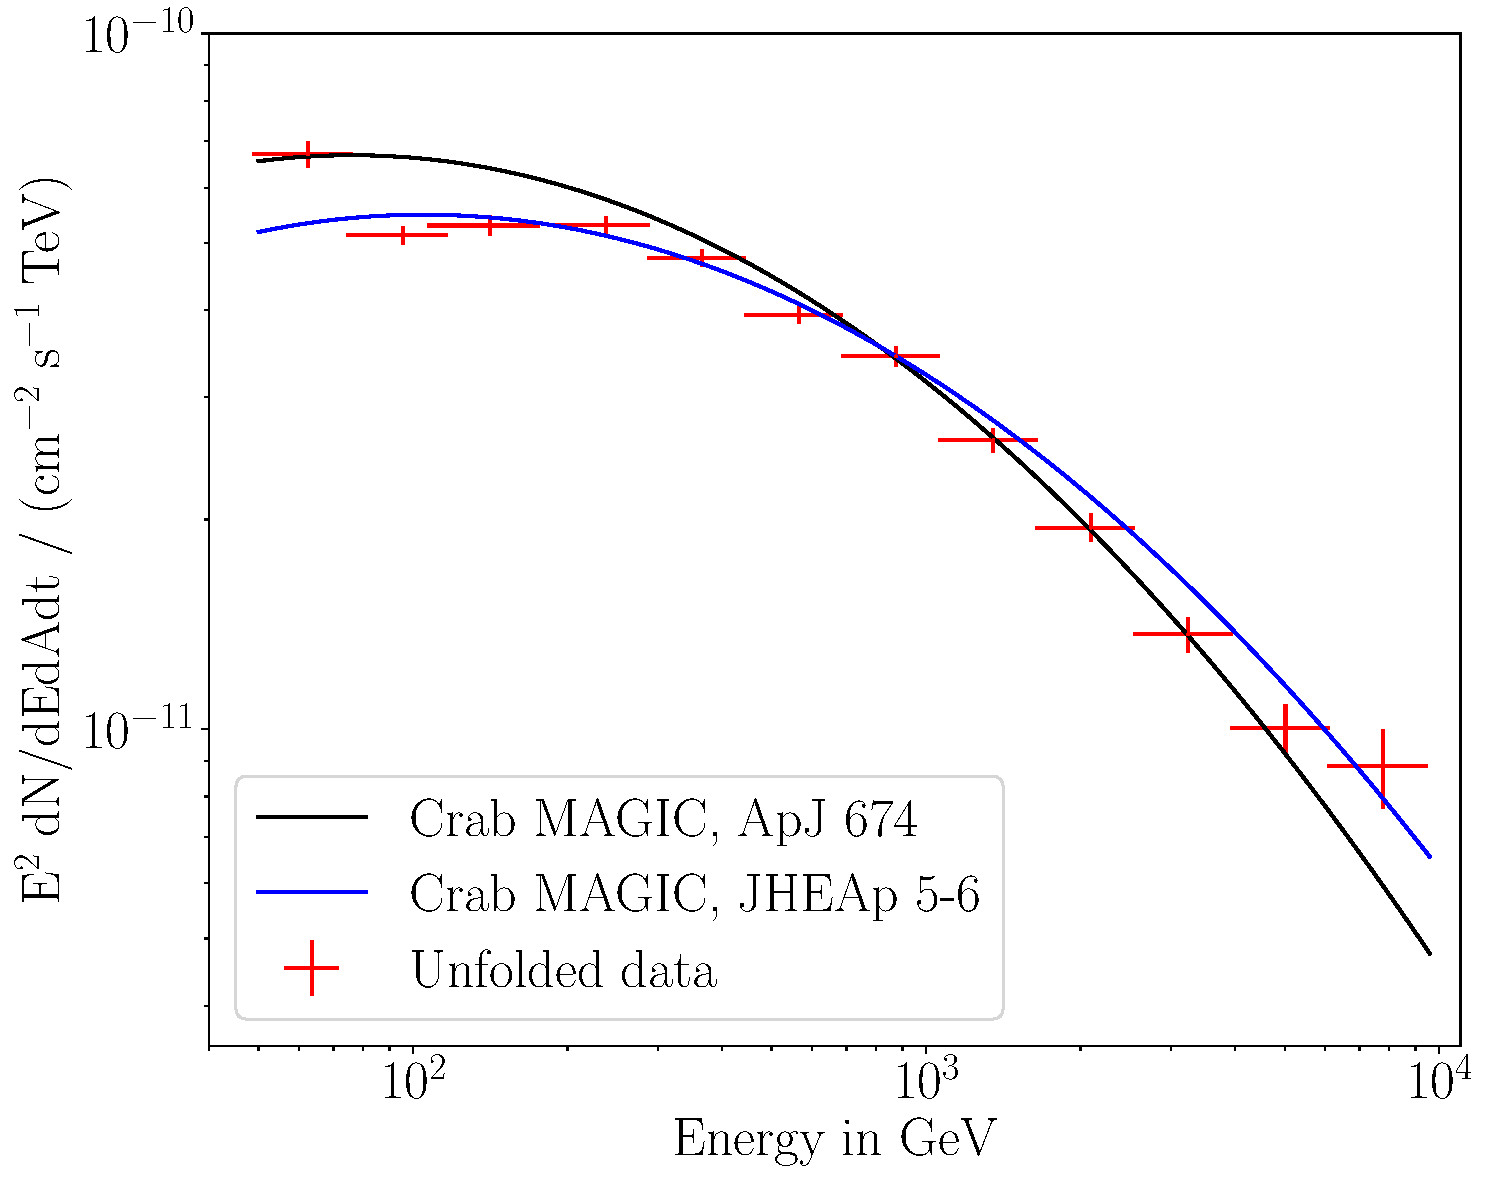
\includegraphics[width=0.8\textwidth]{figures/combunfold_energyspectrum.pdf}
  \caption{Eine Caption.}
\end{figure}
